    \documentclass[letterpaper,11pt]{article}

    \usepackage{fullpage}
    \usepackage[usenames,dvipsnames]{color}
    \usepackage[pdftex]{hyperref}
    \usepackage{tabularx}
\usepackage{booktabs}
\usepackage{amsmath}
\usepackage{multirow}
\usepackage{layouts}
\usepackage{array}
\usepackage{pgf}
\usepackage{tikz}
\usetikzlibrary{positioning}
\usetikzlibrary{arrows,automata}
 \usepackage{graphicx}

   
\begin{document}

\begin{center}
\Huge \textbf{Information Retrieval}\\ \vspace{0.4cm}
\huge \textbf{Lab Assignment 2}\\ \vspace{0.4cm}
\LARGE \textbf{Paris Mavromoustakos (10407502)}\\
\LARGE \textbf{Partick De Kok (5640318)}\\ \vspace{0.4cm}
\textbf{ December 2, 2012}
\end{center}


\section{Introduction}
In the second lab assignment, the goal is to run a small scale IR experiment. That includes a proposal (hypothesis) and the evaluation of TREC's results. In comparison with Assignment 1, we will now emphasize on the interpretation of the output our experiment gives us, rather than the indexing/querying procedure itself. What we expect to obtain from this Assignment is knowledge on how to analyze and evaluate results after running a TREC experiment.


\section{Description of the Data }

For this experiment we use CSIRO document collections, which are pre-processed and ready to be indexed (trectext format). In this case, the documents consist of website content regarding scientific topics. The collection consists of four parts; Corpus.body is the body of the web pages, corpus.title contains the websites' titles, corpus.metadata and corpus.headers contain the metadata and headers of the web pages. 

Moreover, we have 50 TREC Enterprise 2007 topics, which we will apply on our index as Indri queries. Lastly, the relevance assessments file (qrels) is also given and will be used to evaluate the querying output using trec\_eval.9.0.

In this experiment we use porter stemming and there is no stopword removal.



\section{Hypothesis}

We want to compare 3 different but closely related retieval models, BM25, BM15 and BM11. The research questions are "Which one of these models performs better?" and "Does one model perform better over all topics or are there per-topic differences, and why?". Before we hypothesize, we find it important to point out the difference between the 3 retrieval models.

BM(Best Match) 25 is a bag-of-words retrieval function that ranks a set of documents based on the query terms appearing in each document, regardless of the inter-relationship between the query terms within a document[1]. BM25 was created as a combination of the BM11 and BM15 formulas[2] and uses the following formula when computing a document's score:  
\newpage
$Score(D,Q) = \sum^n_{i=1}{IDF(q_i)} \times 	\frac{f(q_i,D) \times (k_1 +1)}{f(q_i,D) + k_1 \times (1-b+b\times \frac{|D|}{avgdl})}$

Where  $f(q_i,D)$ is $q_i$'s term frequency in document D, $|D|$ is document D's length and $avgdl$ is the average document length in the collection. $k_1$ and $b$ are free parameters, with $k_1 \in [1.2,2]$ and $b \in [0,1]$[2]. 



As we can see from the formula above, the term $b$ plays an important role as it defines the importance of document length[3]: $b=1$ means we fully scale the term weight by document length and our the retrieval model transforms into BM11[2], while $b=0$ means the document length is not taken into consideration (BM15[2]).

BM25's default value for $b$ is 0.75,and additionally for $k_1$ 1.25 is considered a reasonable value[1]. In this experiment, we keep the default value for $k_1$ and use the 3 different values of $b$ mentioned above.

After studying the 3 retrieval models we hypothesize that BM25 will outperform BM11 and BM15 both on recall and MAP, for the reason that it "balances" between the other two models aiming towards optimization based on the document length factor. We believe that the extreme values of 0 and 1 for $b$ will give different but still worse results than those of $b=0.75$, both over all topics, and even per-topic. More, experiments have shown that BM11 outperforms BM15[2], so we expect BM11 to be the second-to-best model regarding performance.




\section{Related Work}

Numerous books and articles mention the BM25 retrieval model as a combination of BM11 and BM15. "Introduction to Information Retrieval"  (Christopher D. Manning, Prabhakar Raghavan \& Hinrich Schütze, 2008) discuss BM25 as a probabilistic information retrieval model and mention the different possible values for the $b$ term. 

A deeper comparison between the three retrieval models is made in "Modern Infromation Retrieval" (Ricardo Baeza-Yates, Berthier Ribeiro-Neto, 2006) where the BM25 formula is analyzed in detail. In this book, discussion is presented about the suggested values for $k_1$ and $b$ and how changing these values affects the model. 



\section{Experimenting results}

In this section we will present the results of our experiment, divided in two sections; results over all topics and some examples of per-topic results. Discussion and conclusions over the results will be presented in the next chapters.

\subsection{Results over all topics}


Results over  all topics are necessary to observe the general behavior of the models. Below we present important results over metrics that describe the 3 different models' average performances.


\begin{center}
\begin{table}[ht]
\centering
\begin{tabular}{c | c c c}
   & BM11  & BM25 & BM15  \\  \hline
MAP & 0.3491 & 0.4035 & 0.3068 \\
Num\_rel\_ret & 4628 & 4738 & 4478 \\
R-precision & 0.3728 & 0.4138 & 0.3402
\end{tabular}
\caption{Metrics over all topics}  
\end{table}
\end{center}

\vspace{5cm}
\begin{figure}[h]
\centering
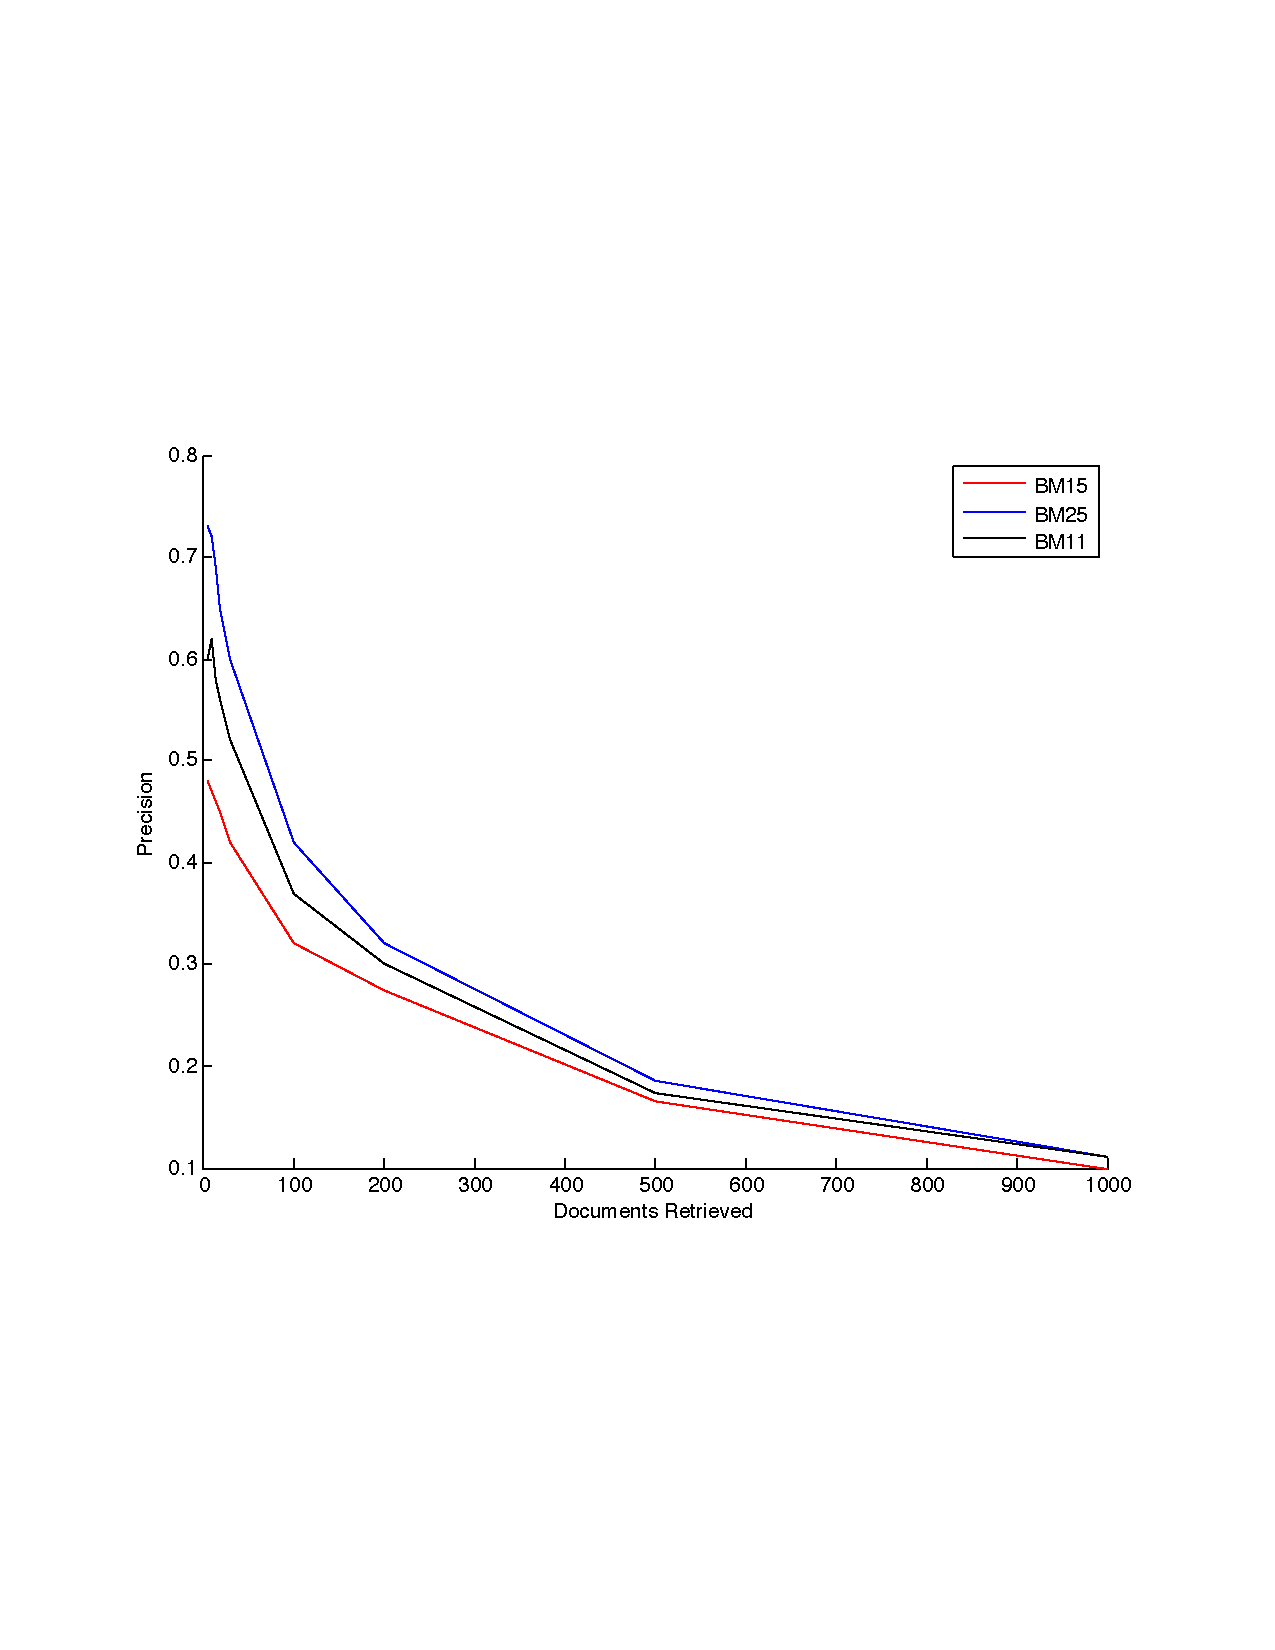
\includegraphics[scale = 0.75]{dr.pdf}
\caption{Precision after 5, 10, \dots, 1000 documents retrieved over all topics}

\end{figure}

\newpage 


\begin{figure}[ht]
\centering
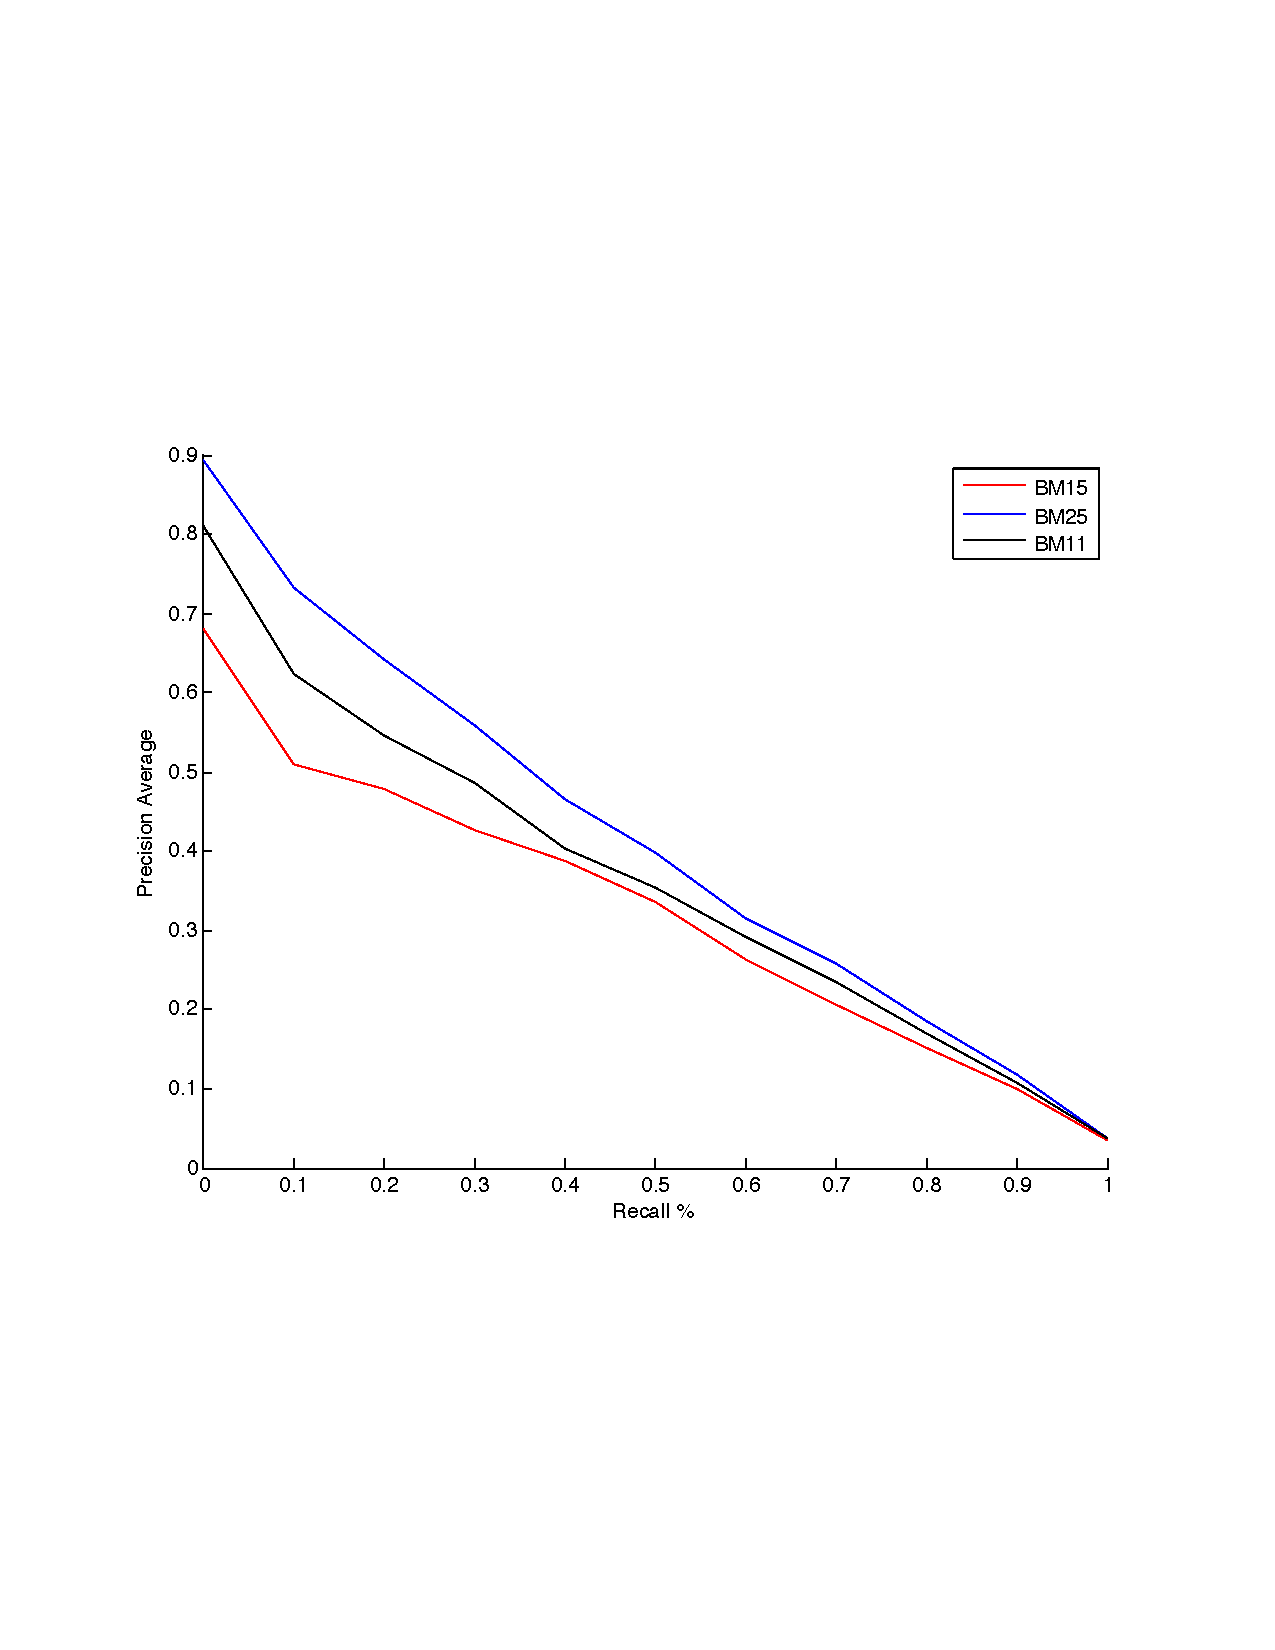
\includegraphics[scale = 0.75]{pr.pdf}
\caption{Precision - Recall curve over all topics}

\end{figure}



\subsection{Per-topic results}

Per-topic results will be presented in this section, in order to examine the models' behavior deeper into detail and point out interesting observations. Of course, it is not possible to discuss each query one by one, so we will be examining those which we find important for our analysis.

Below we present some metrics calculated from the 3 models over query No. 1 ("genetic modification"): 



\begin{center}
\begin{table}[ht]
\centering
\begin{tabular}{c | c c c}
   & BM11  & BM25 & BM15  \\  \hline
MAP & 0.3491 & 0.4035 & 0.3068 \\
Num\_rel\_ret & 133 & 124 & 113 \\
R-precision & 0.2418 & 0.2381 & 0.2088
\end{tabular}
\caption{Metrics over query No. 1}  
\end{table}
\end{center}

\newpage

The same metrics calculated over query No. 14 ("high protein diet"):


\begin{center}
\begin{table}[ht]
\centering
\begin{tabular}{c | c c c}
   & BM11  & BM25 & BM15  \\  \hline
MAP & 0.3932 & 0.4242 & 0.3507 \\
Num\_rel\_ret & 68 & 70 & 63 \\
R-precision & 0.3733 & 0.4000 & 0.3467
\end{tabular}
\caption{Metrics over query No. 14}  
\end{table}
\end{center}

\begin{figure}[h]
\centering
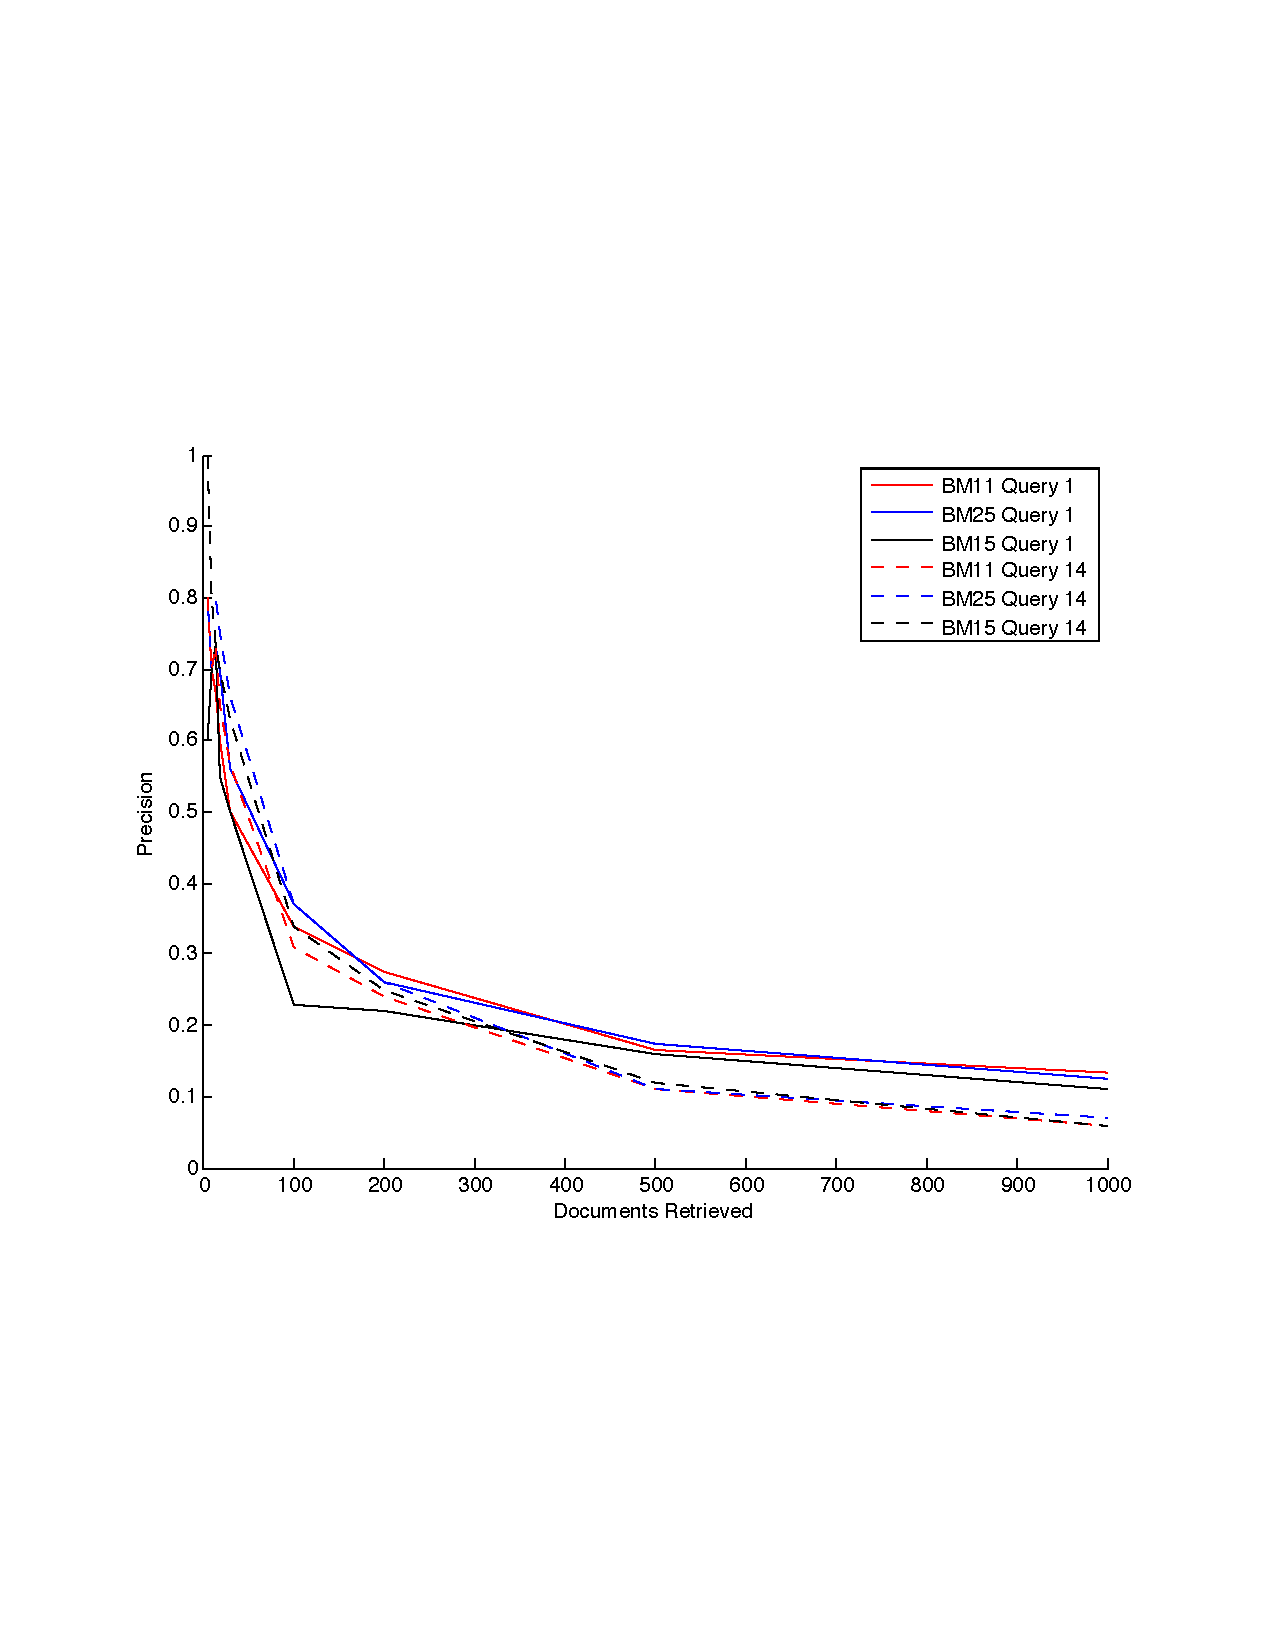
\includegraphics[scale = 0.75]{dr2.pdf}
\caption{Precision over 5, 10, \dots, 1000 documents retrieved on queries 1\& 14}

\end{figure}

\newpage

\section{Discussion}
Table 1 and Figure 1 show us that BM25 clearly dominates BM11 and BM15 on both MAP and Recall over all topics. After having observed these results we can now confidently state that BM25 is a "version" of combined BM11 and BM15 that optimizes performance. Moreover, comparing BM11 and BM15, it is obvious that BM11 performs significantly better. 

Per-topic results indicate better performance for BM25 regarding MAP, however, in the two examples of the previous chapter we can see that BM11 performs as well as (or even better than) BM25 on certain queries, regarding Recall. We believe that these results can be obtained by queries which are related to small-size documents. As derived from the formula presented in chapter 3, smaller documents increase the score of queries related to them. And while in BM11 we consider the document size to be of more importance than in BM25, there is a chance BM11 can come up with higher scores than BM25. Again, BM15 can clearly be considered as the worst performing model.



\section{Conclusion}

Regarding our hypothesis, the fact is that results over all topics confirm our prior beliefs. BM25 performs better than the other 2 models on all metrics examined, while BM11 dominates BM15 as stated in [2]. More, per-topic results aswell show us that our hypothesis was correct, even though the difference we observe between BM25 and BM11 is smaller than expected, and BM11 does occasionaly outperform BM25.

We can now answer the questions of chapter 3 and say that BM25 performs better than the other two models over all topics, while applying BM11 over certain topics is sometimes the best choice regarding Recall.


\begin{thebibliography}{9}
\bibitem{wikipedia}
\emph{www.wikipedia.org}
\bibitem{MIR}
  Ricardo Baeza-Yates \& Berthier Ribeiro-Neto,
   \emph{Modern information Retrieval}.
  Addison Wesley,
  2006.
  \bibitem{IIR}
  Christopher D. Manning, Prabhakar Raghavan \& Hinrich Schütze,
  \emph{Introduction to Information Retrieval}.
  Cambridge University Press,
  2008.



\end{thebibliography}

    \end{document}


